\chapter{Wdrożenie i prezentacja działania}
\thispagestyle{chapterBeginStyle}

W tym rozdziale została przedstawiona instrukcja obsługi niniejszej platformy. W pierwszej części omówiono wymagania, które muszą zostać spełnione, aby framework z przykładowymi danymi był gotów do pracy, następnie opisano czynności instalacyjne. 
W dalszej części rozdziału umieszczono prezentację działania aplikacji.  

%W tym rozdziale należy omówić zawartość pakietu instalacyjnego oraz założenia co do środowiska, w którym realizowany system będzie instalowany. Należy przedstawić procedurę instalacji i wdrożenia systemu. Czynności instalacyjne powinny być szczegółowo rozpisane na kroki. Procedura wdrożenia powinna obejmować konfigurację platformy sprzętowej, OS (np. konfiguracje niezbędnych sterowników) oraz konfigurację wdrażanego systemu, m.in.\ tworzenia niezbędnych kont użytkowników. Procedura instalacji powinna prowadzić od stanu, w którym nie są zainstalowane żadne składniki systemu, do stanu w którym system jest gotowy do pracy i oczekuje na akcje typowego użytkownika.%
\section{Konfiguracja i instalacja aplikacji}
Aplikację można uruchomić na każdym systemie, na którym jest możliwa instalacja bazy danych PostgreSQL. Najprościej pobrać jej obraz z repozytorium Docker-Hub i uruchomić aplikacją Docker. Przykładowa instalacja odbędzie się na przykładzie komputera z systemem Ubuntu 16.04. 

\subsubsection{Instalacja Javy}
Javę na Ubuntu 16.04 wystarczy zainstalować za pomocą polecenia:

\noindent
\texttt{\$ sudo apt-get install default-jdk}

\noindent
Na nowszych wersjach Ubuntu należy zainstalować Javę 8, ponieważ pakiet \texttt{default-jdk} zawiera Javę 10. W tym celu należy pobrać ze strony \cite{Java-doc} paczkę z Javą 8 i ustawić zmienną środowiskową \texttt{JAVA\_HOME} na miejsce wypakowania paczki. 

\subsubsection{Instalacja Dockera}
Docker na Ubuntu jest bardzo prosty w instalacji, pełny (pięciominutowy) poradnik znajduje się pod adresem \cite{docker-ins}.

\subsubsection{Instalacja bazy danych PSQL}
Obraz bazy danych zostanie pobrany przez aplikację Docker po wpisaniu poniższej komendy: 

\noindent
\texttt{\$ docker run --name postgres -e POSTGRES\_PASSWORD=postgres -d postgres}

\subsubsection{Skrypty tworzące użytkownika i bazę danych}
W głównym folderze pakietu instalacyjnego należy odszukać katalog \textbf{sql} i uruchomić skrypty \texttt{1.sql, 2.sql, 3.sql, 4.sql} na postawionej w poprzednim kroku bazie danych.

\subsubsection{Serwer Apache Solr}
Serwer Apache Solr również zostanie pobrany z obrazu Docker'owego. Aby uruchomić instancję Apache Solr na komputerze należy wpisać polecenie: 

\noindent
\texttt{\$ docker run --name my\_solr -d -p 8983:8983 -t solr}



\subsubsection{Instalacja aplikacji testowej}
W głównym folderze pakietu instalacyjnego znajdują się dwie paczki: \texttt{admin.jar} oraz \texttt{shop.jar}. Obydwie należy uruchomić za pomocą polecenia: 

\noindent
\texttt{\$ java -jar nazwa.jar}

\noindent
gdzie \textit{nazwa} to \textit{admin} lub \textit{shop}. Sklep z wszystkimi produktami będzie dostępny pod adresem http://localhost:9001/search?query=*, natomiast panel administracyjny z wylistowanymi kategoriami pod adresem http://localhost:9000/entities/category. System administracyjny będzie wymagał zalogowania. Dane do logowania: \texttt{login: admin, hasło: test}. Aby zakupić przedmiot w sklepie, również są potrzebne dane do logowania: \texttt{login: test, hasło: test}

\section{Prezentacja działania}
W ramach tej sekcji zostaną przedstawione kluczowe elementy systemu, które pojawiły się w rozdziale \textbf{Projekt systemu}.  

\subsubsection{Widok panelu administracyjnego}
Na rysunku \ref{scr_adminmain} został przedstawiony panel administracyjny. Literkami A, B, C i D oznaczono ważne elementy. \textbf{A} -- konfigurowalne menu, \textbf{B} -- dynamiczna tabela encyjna ze wszystkim encjami rodzaju \texttt{price} (tabela cen). \textbf{C} przycisk dodania nowego egzemplarza encji, \textbf{D} -- linki z ID przekierowują do dynamicznego formularza edycji encji. 
\begin{figure}[h]
	\begin{center}
		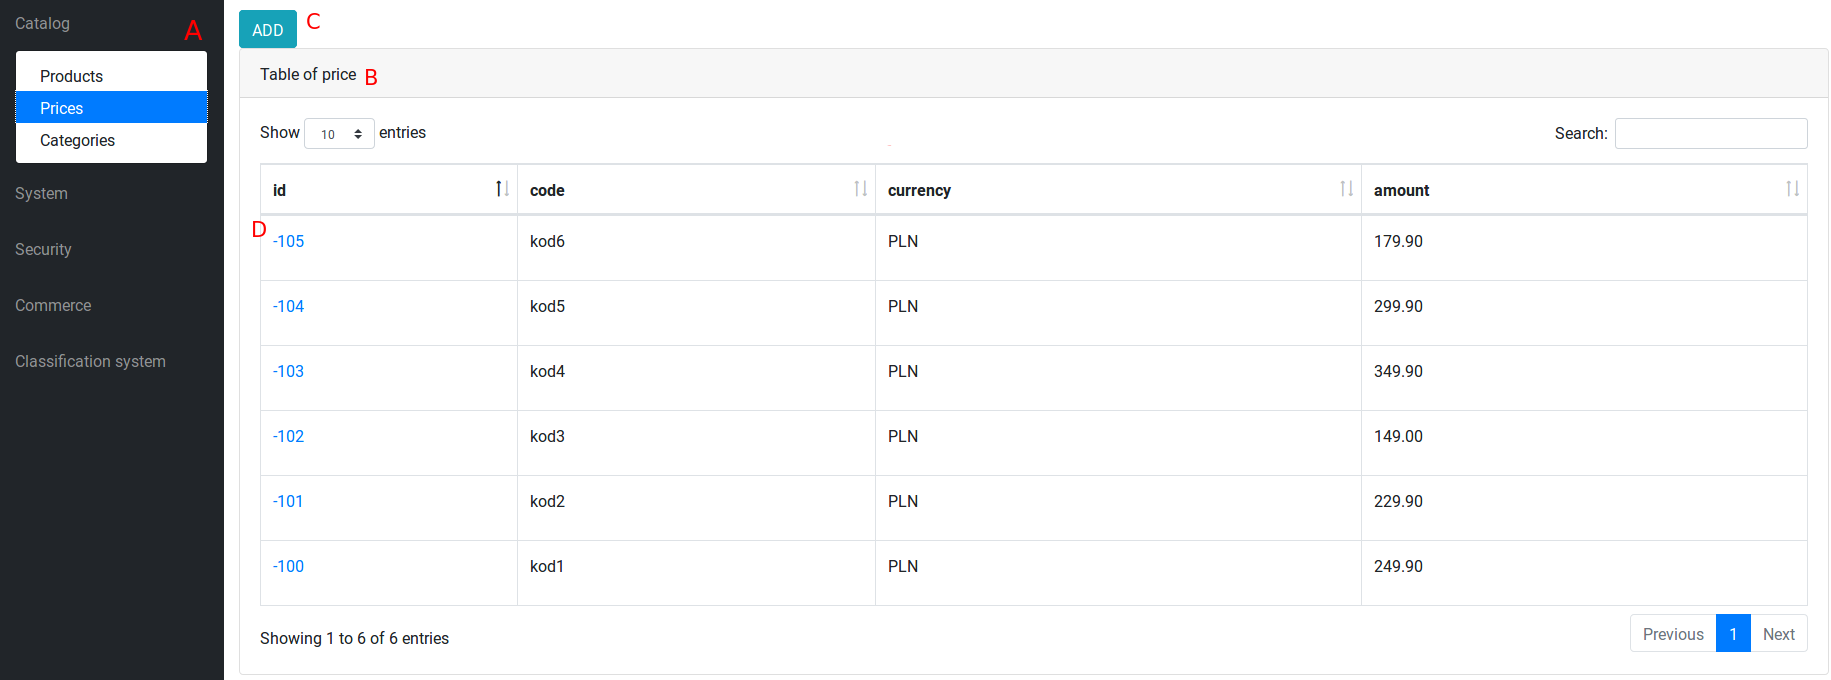
\includegraphics[width=1\textwidth]{admin-main.png}
	\end{center}
	\caption{{\color{black}Widok panelu administracyjnego}} \label{scr_adminmain}
\end{figure}


\subsubsection{Zmiana właściwości encji} 
Zmiana właściwości dowolnej encji zostanie przedstawiona na podstawie produktu.
 
\noindent
\textbf{Scenariusz: } zmiana ceny. \textbf{Rysunek: } \ref{zmianacenyproduktu} 
\begin{itemize}
	\item wybierz z tabeli encyjnej dowolny produkt i wejdź w szczegóły (1)
	\item w dynamicznym formularzu spośród relacji produktu wybierz cenę (price) i wejdź w szczegóły (2) 
	\item w formularzu edycji ceny zmień jej wartość i naciśnij \textit{submit}(3)
	\item po powrocie do edycji produktu zostanie wyświetlona zmieniona cena (4)
\end{itemize}
\begin{figure}
	\begin{center}
		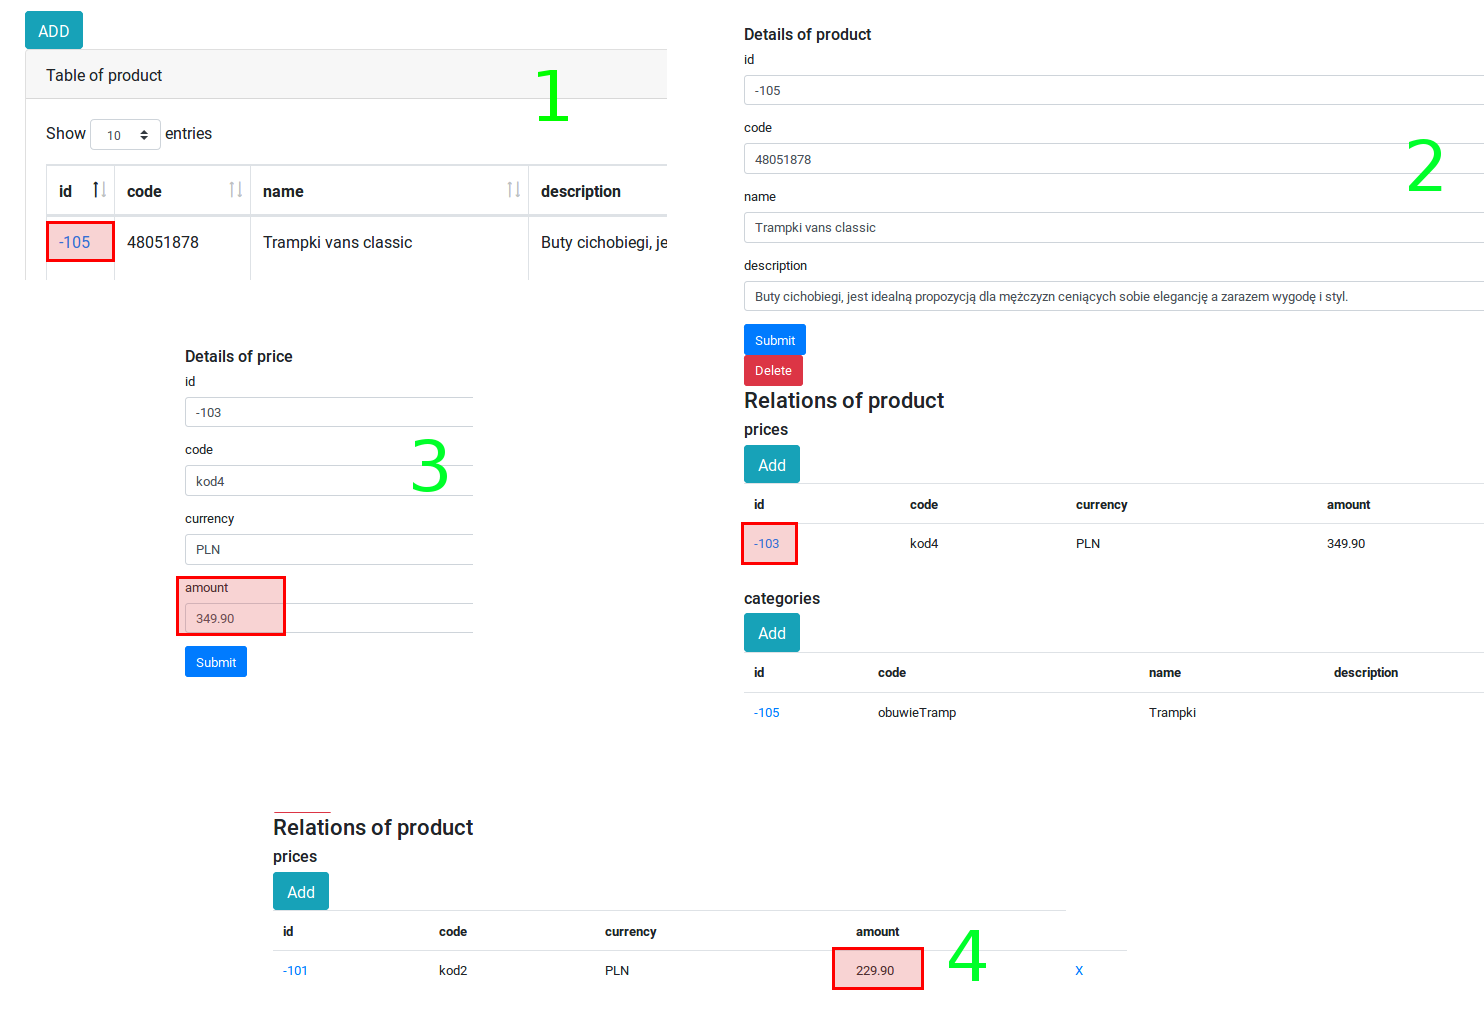
\includegraphics[scale=1.3]{zmianacenyproduktu.png}
	\end{center}
	\caption{{\color{black}Zmiana ceny w produkcie}} \label{zmianacenyproduktu}
\end{figure}









